\documentclass{article}

\usepackage{graphicx}
\usepackage{tikz}
\usepackage{tikzsymbols}
\usetikzlibrary{calc,patterns,shapes.geometric}
\pagestyle{empty}
\usepackage[margin=0pt]{geometry}
\geometry{papersize={14in,12in}}

\def\centerarc[#1](#2)(#3:#4:#5){\draw[#1] ($(#2)+({#5*cos(#3)},{#5*sin(#3)})$) arc (#3:#4:#5);}

\begin{document}
	\begin{figure}
		\centering
		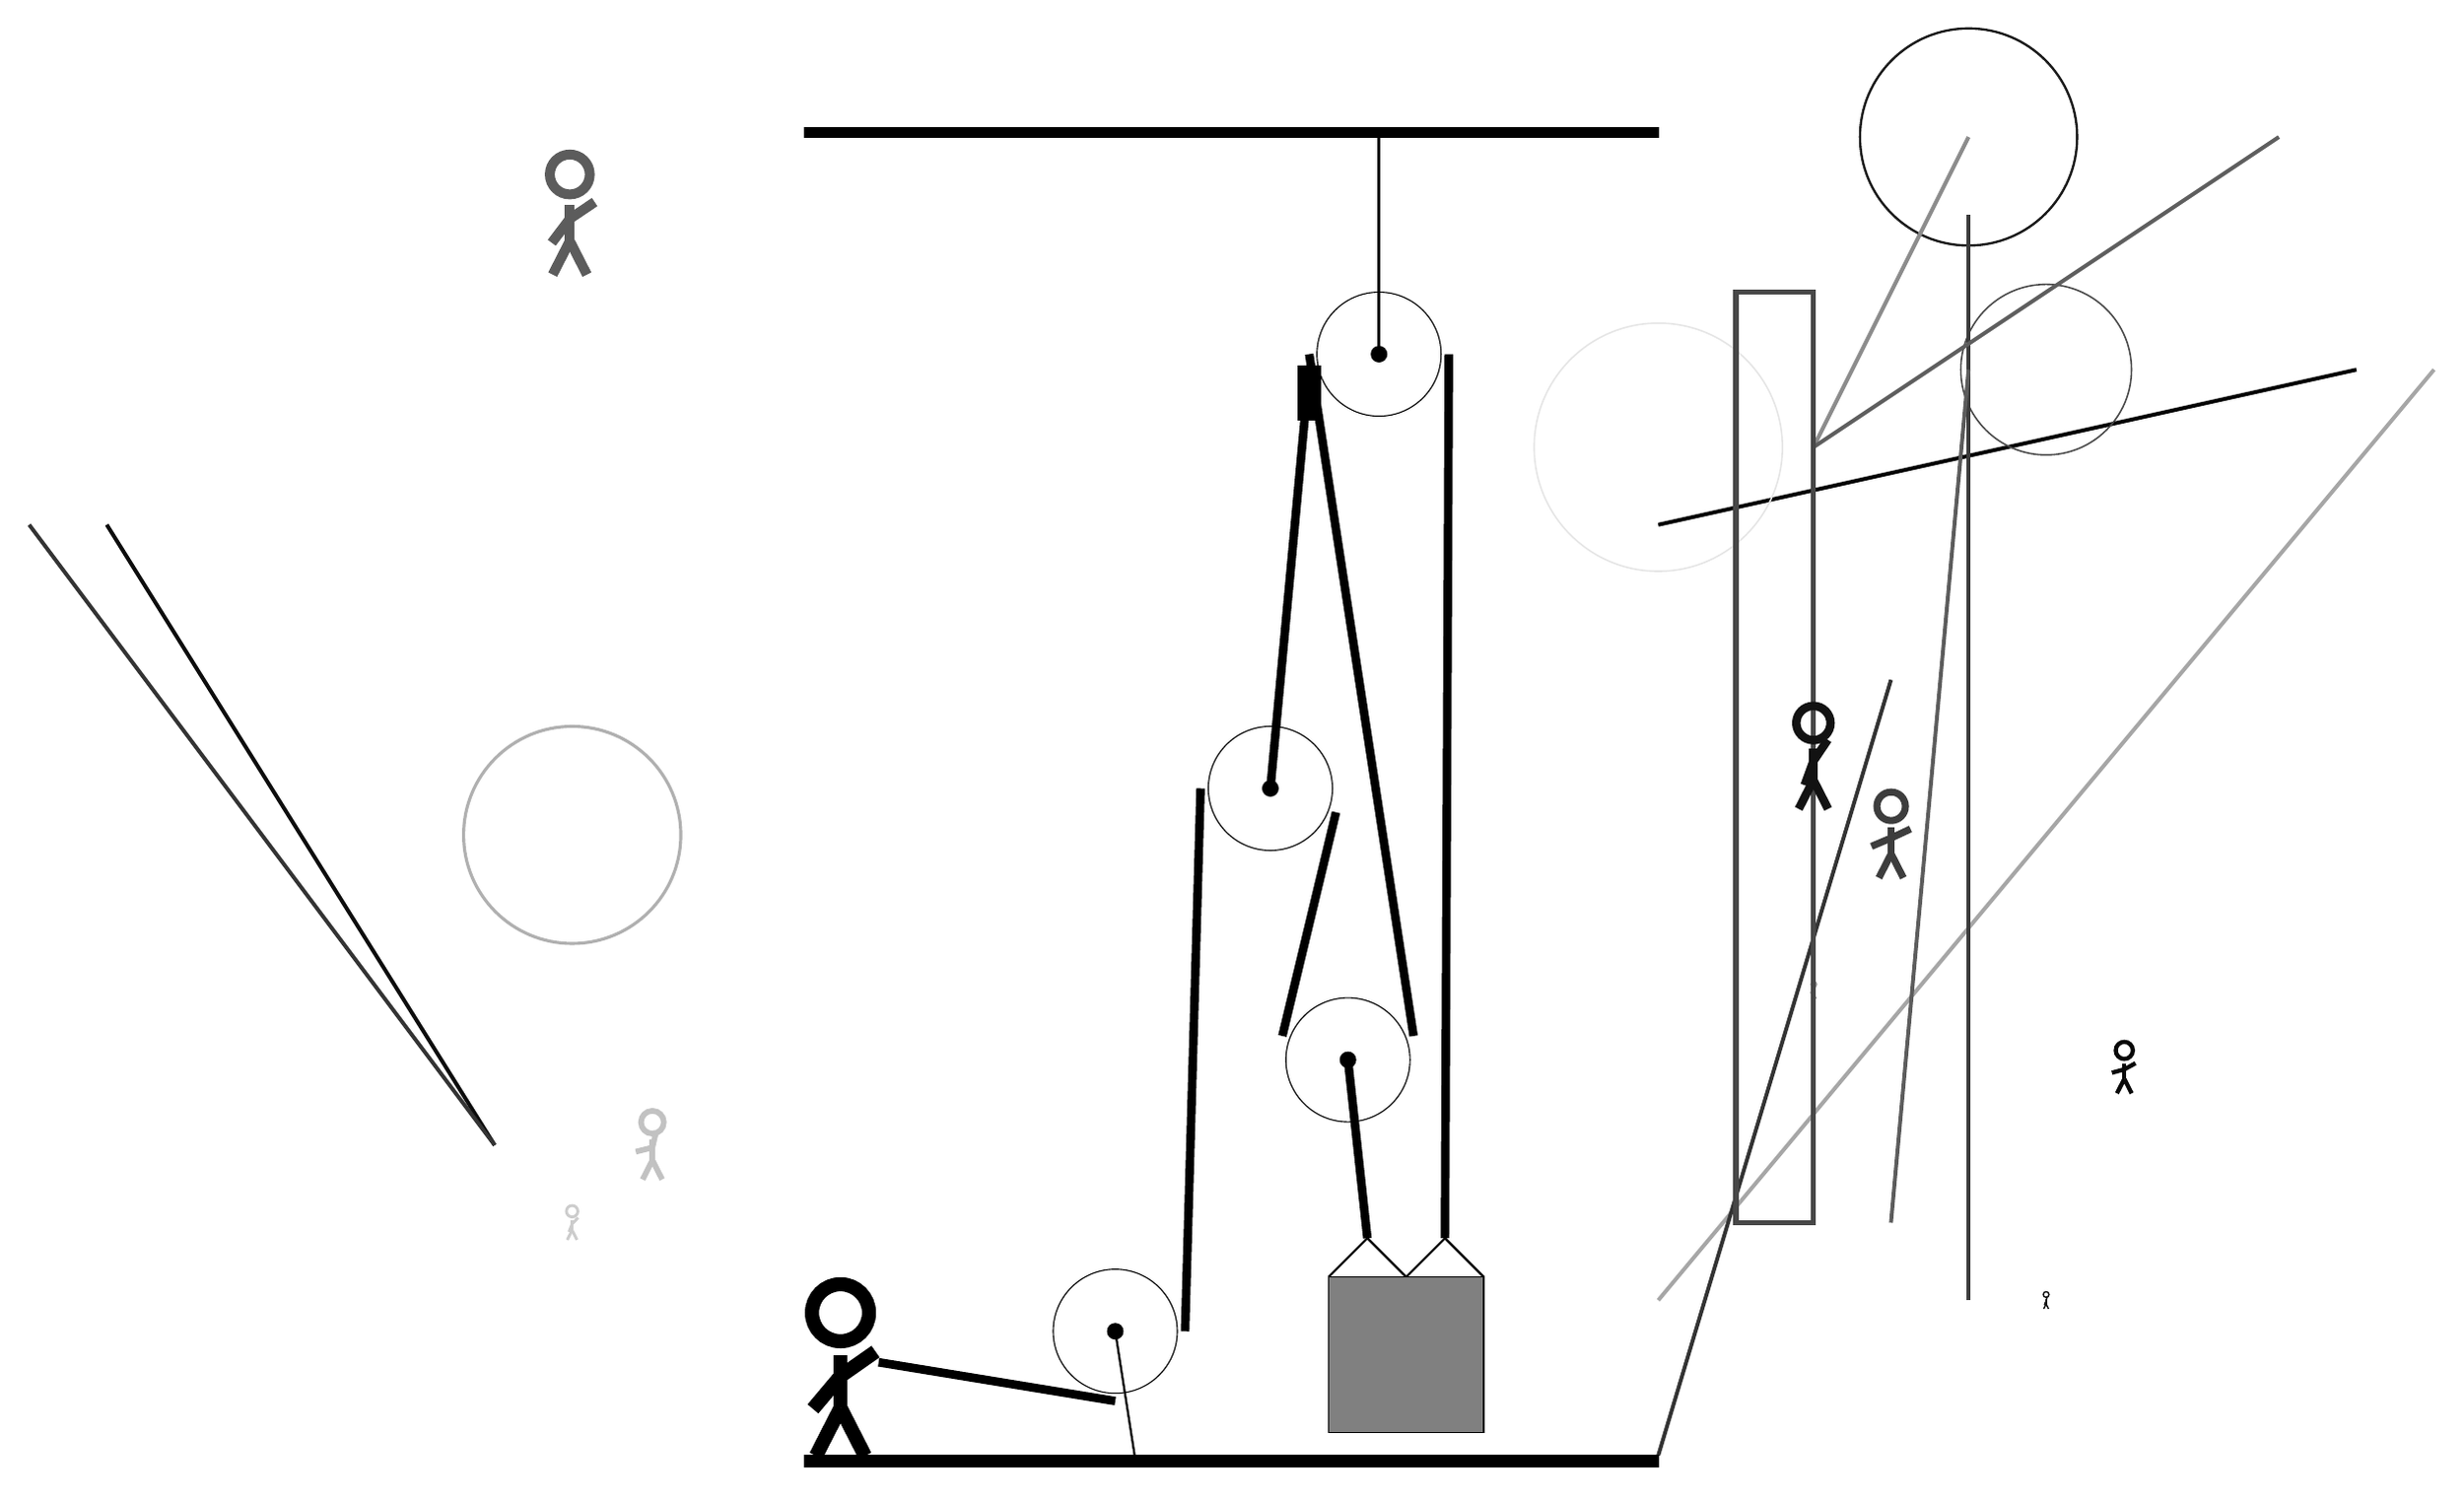
\begin{tikzpicture}
			%%%%% START %%%%%
			
			\draw[fill=black] (-6, 14) rectangle (5, 14.125);
			
			\draw (0, 5.6) circle (0.8);
			\draw[fill=black] (0, 5.6) circle (0.1);
			
			\draw (1, 2.1) circle (0.8);
			\draw[fill=black] (1, 2.1) circle (0.1);
			
			\draw (1.4, 11.2) circle (0.8);
			\draw[fill=black] (1.4, 11.2) circle (0.1);
			\draw[very thick] (1.4, 11.2) -- (1.4, 14);
			
			\draw[line width=0.5mm, color=black!100](5, 9) -- (14, 11);
			
			\node[line width=0.7mm, color=black!97] at (11, 2) {\Strichmaxerl[3][15][29]};
			\draw[line width=0.5mm, color=black!95](-10, 1) -- (-15, 9);
			\draw [line width=0.2mm, color=black!10](5, 10) circle (1.6);
			\node[line width=0.4mm, color=black!76] at (8, 5) {\Strichmaxerl[5][23][25]};
			\draw[line width=0.5mm, color=black!35](5, -1) -- (15, 11);
			
			\node[line width=0.3mm, color=black!40] at (7, 3) {\Strichmaxerl[1][34][67]};
			\draw [line width=0.3mm, color=black!90](9, 14) circle (1.4);
			\draw [line width=0.4mm, color=black!31](-9, 5) circle (1.4);
			
			\draw [line width=0.2mm, color=black!71](10, 11) circle (1.1);
			\draw[line width=0.5mm, color=black!80](5, -3) -- (8, 7);
			\draw[line width=0.5mm, color=black!77](9, -1) -- (9, 13);
			\node[line width=0.6mm, color=black!64] at (-9, 13) {\Strichmaxerl[7][53][34]};
			
			\node[line width=0.5mm, color=black!24] at (-8, 1) {\Strichmaxerl[4][14][77]};
			\draw[line width=0.5mm, color=black!45](7, 10) -- (9, 14);
			\draw[line width=0.5mm, color=black!64](9, 11) -- (8, 0);
			
			\node[line width=0.6mm, color=black!20] at (-9, 0) {\Strichmaxerl[2][68][46]};
			\draw[line width=0.5mm, color=black!63](7, 10) -- (13, 14);
			\draw[line width=0.7mm, color=black!72] (7, 12) rectangle (6, 0);
			\node[line width=0.4mm, color=black!92] at (10, -1) {\Strichmaxerl[1][66][76]};
			\node[line width=0.3mm, color=black!93] at (7, 6) {\Strichmaxerl[6][70][56]};
			\draw[line width=0.5mm, color=black!80](-10, 1) -- (-16, 9);
			
			\draw (-2, -1.4) circle (0.8);
			\draw[fill=black] (-2, -1.4) circle (0.1);
			\draw[thick] (-2, -1.4) -- (-1.75, -3);
			
			
			\draw[thick]  (0.75, -0.7) -- (1.25, -0.2) -- (1.75, -0.7) -- (2.25, -0.2) -- (2.75, -0.7);
			\draw[fill=black!50] (0.75, -0.7) rectangle (2.75, -2.7);
			\draw[line width=1.1mm] (-5.05, -1.8) -- (-2, -2.3);
			\centerarc[line width=1.1mm](-2, -1.4)(270:360:0.9);
			\draw[line width=1.1mm] (-1.1, -1.4) -- (-0.9, 5.6);
			\draw[line width=1.1mm] (0, 5.6) -- (0.5, 11.0);
			\draw[line width=1.1mm, fill=black](0.4, 10.4) rectangle (0.6, 11.0);
			\centerarc[line width=1.1mm](0, 5.6)(-20:180:0.9);
			\draw[line width=1.1mm] (0.8457, 5.2922) -- (0.1543, 2.4078);
			\centerarc[line width=1.1mm](1, 2.1)(160:380:0.9);
			\draw[line width=1.1mm] (1.8457, 2.4078) -- (0.5, 11.2);
			\draw[line width=1.1mm](1, 2.1) -- (1.25, -0.2);
			\centerarc[line width=1.1mm](1.4, 11.2)(0:180:0.9);
			\draw[line width=1.1mm] (2.3, 11.2) -- (2.25, -0.2);
			
			\node at (-5.5, -1.9) {\Strichmaxerl[10][50][35]};
			
			\draw[fill=black] (-6, -3) rectangle (5, -3.15);
			
			%%%%% END %%%%%
		\end{tikzpicture}
	\end{figure}	
\end{document}